\documentclass[12pt]{article}
\usepackage[english]{babel}
\usepackage{array}
\usepackage{setspace}
\usepackage{graphicx}
\usepackage{sistyle} %\num{100000} for commas
\SIthousandsep{,}
\usepackage{fancyhdr}
\usepackage{listings} % For code listings, may break stuff
\usepackage{xcolor, diagbox, empheq, makecell, tcolorbox}
\usepackage[autostyle]{csquotes}
\usepackage{amssymb, amsthm, linguex, enumitem, amsmath}
\usepackage{tcolorbox} %dont know what this does
\usepackage[colorlinks=true, allcolors=blue]{hyperref}
\usepackage{lipsum}
\usepackage{notomath}
\usepackage[T1]{fontenc}
\makeatletter   %% <- make @ usable in macro names
\newcommand*\notab[1]{%
  \begingroup   %% <- limit scope of the following changes
    \par        %% <- start a new paragraph
    \@totalleftmargin=0pt \linewidth=\columnwidth
    %% ^^ let other commands know that the margins have been reset
    \parshape 0
    %% ^^ reset the margins
    #1\par      %% <- insert #1 and end this paragraph
  \endgroup
}
\makeatother    %% <- revert @

\pagestyle{empty}

\textwidth 6.5in
\hoffset=-.65in
\textheight=9.5in
\voffset=-1.in

%Sets
\newcommand{\R}{\mathbb{R}}
\newcommand{\C}{\mathbb{C}}
\newcommand{\N}{\mathbb{N}}
\newcommand{\F}{\mathbb{F}}
\newcommand{\Z}{\mathbb{Z}}
\newcommand{\Cb}{\mathbf{C}}
\newcommand{\Fb}{\mathbf{F}}
\newcommand{\Rb}{\mathbf{R}}

%Misc

\newcommand{\pars}[1]{\left( {#1} \right) } %auto size parenthesis 
\newcommand{\brac}[1]{\left[ {#1} \right] } %auto size brackets around arg
\newcommand{\set}[1]{\left\{{#1}\right\}} %auto size curly braces around arg
\newcommand{\vbrac}[1]{\left\langle{#1}\right\rangle} %vector angle brackets
\newcommand{\inner}[1]{\left\langle{#1}\right\rangle} %vector angle brackets
\newcommand{\conj}[1]{\overline{{#1}}} %conjugate bar
\newcommand{\vconj}[1]{\overline{\vbrac{{#1}}}}
\newcommand{\ceil}[1]{\left\lceil {#1} \right\rceil} %auto size ceiling around arg
\newcommand{\floor}[1]{\left\lfloor {#1} \right\rfloor} %auto size floor around arg

\newcommand{\limn}{\lim_{n\to\infty}} %limit as n approaches infinity
\newcommand{\thru}[1]{{#1}_1, \dots, {#1}_n}
\newcommand{\sumthru}[1]{{#1}_1 + \cdots + {#1}_n}
\renewcommand{\over}[1]{\frac{1}{{#1}}}
\newcommand{\pfrac}[2]{\left( \frac{{#1}}{{#2}} \right) } %auto size parenthesis over fraction 
\newcommand{\pdfrac}[2]{\left( \dfrac{{#1}}{{#2}} \right) } %auto size parenthesis over fraction 
\newcommand{\pover}[1]{\left( \frac{1}{{#1}} \right) } %auto size parenthesis over fraction

%Boolean Algebra
\newcommand{\OR}{\,\lor\,}
\newcommand{\AND}{\,\land\,}

%Probability and Statistics
\newcommand{\xbar}{\bar{X}}
\newcommand{\ybar}{\bar{Y}}
\newcommand{\yn}{Y_1, \dots, Y_n}
\newcommand{\yx}{X_1, \dots, X_n}
\newcommand{\normDist}{N\left(\mu, \sigma^2\right)} %default normal distribution
\newcommand{\gammaDist}[2]{\operatorname{Gamma} \left( {#1},{#2} \right)}
\newcommand{\norm}[1]{\left\| {#1} \right\|}
\newcommand{\abs}[1]{\left| {#1} \right|}
\newcommand{\prob}[1]{P \left( {#1} \right) }
\newcommand{\E}[1]{E \left( {#1} \right) }
\newcommand{\Eb}[1]{E[ \,{#1}\, ]} %E bracket
\newcommand*{\V}[1]{V \left( {#1} \right) }
\newcommand{\Vb}[1]{V [ \,{#1}\, ] }
\newcommand{\that}{\hat{\theta}} %theta hat
\newcommand{\phat}{\hat{p}}
\newcommand{\psihat}{\hat{\psi}}
\newcommand{\Psihat}{\hat{\Psi}}


\newcommand{\dimrange}[1]{\operatorname{dim}\operatorname{range}{#1}} % dimrange
\newcommand{\dimnull}[1]{\operatorname{dim}\operatorname{null}{#1}} % dimnull

\newcommand{\vdub}[2]{\begin{pmatrix}{#1}\\{#2}\end{pmatrix}}

%Linear Algebra
\newcommand{\poly}[1]{\mathcal{P}_{#1}(\mathbf{R})} %polynomial up to degree (arg)
\newcommand{\pf}{\mathcal{P}(\mathbf{F})} %set of all polynomials
\renewcommand{\L}[1]{\mathcal{L}\left({#1}\right)}%Set of linear maps
\newcommand{\vdouble}[2]{\begin{pmatrix}{#1}\\{#2}\end{pmatrix}} % 2 high vertical
\newcommand{\vtriple}[3]{\begin{pmatrix}{#1}\\{#2}\\{#3}\end{pmatrix}} %vertical vector parenthesis, 3 args
\newcommand{\vquad}[4]{\begin{pmatrix}{#1}\\{#2}\\{#3}\\{#4}\end{pmatrix}} %vertical vector parenthesis, 4 args
\newcommand{\vquin}[5]{\begin{pmatrix}{#1}\\{#2}\\{#3}\\{#4}\\{#5}\end{pmatrix}} %vertical vector parenthesis, 5 args
\newcommand{\vvector}[3]{\begin{bmatrix}{#1}\\{#2}\\{#3}\end{bmatrix}} %vertical vector braces, 3 args
\newcommand{\dimn}[1]{\operatorname{dim}\,{#1}}
\newcommand{\rank}[1]{\operatorname{dim}\operatorname{range}{#1}}
\newcommand{\nullity}[1]{\operatorname{dim}\operatorname{null}{#1}}
\newcommand{\range}[1]{\operatorname{range}{#1}}
\newcommand{\NULL}[1]{\operatorname{null}{#1}}
\renewcommand{\null}{\operatorname{null}}
\newcommand{\mat}[4]{\begin{bmatrix}{#1} & {#2}\\{#3}&{#4}\end{bmatrix}} % 2x2 matrix
\newcommand{\Mat}[9]{\begin{bmatrix}{#1} & {#2} & {#3}\\{#4}&{#5}&{#6}\\{#7}&{#8}&{#9}\end{bmatrix}} % 3x3 matrix
\newcommand{\detx}[4]{\begin{vmatrix}{#1} & {#2}\\{#3}&{#4}\end{vmatrix}} % 2x2 determinant
\newcommand{\nf}{\infty}
%colors
\definecolor{ggreen}{RGB}{0, 127, 0}
\definecolor{dgray}{RGB}{63,63,63}
\definecolor{neonorange}{RGB}{255,47,0}
\definecolor{mygray}{rgb}{0.5,0.5,0.5}
\newcommand{\red}[1]{\color{red}{#1}\color{black}}
\newcommand{\grn}[1]{\color{ggreen}{#1}\color{black}}
\newcommand{\blu}[1]{\color{blue}{#1}\color{black}}
\newcommand{\redx}[1]{\color{red}\not{#1}\color{black}}

\newcommand{\say}[1]{\textquotedblleft{#1}\textquotedblright} %quote the "argument"
\newcommand*\widefbox[1]{\fbox{\hspace{2em}#1\hspace{2em}}}
\newtcolorbox{mybox}[1][]{colback=white, sharp corners, #1}

%Line break spacings
\newcommand{\nl}{\vspace{0.1in}\noindent}
\newcommand{\nnl}{\vspace{0.2in}\noindent}
\newcommand{\nnnl}{\vspace{0.3in}\noindent}

% Code snippets
\newcommand*{\code}{\fontfamily{qcr}\selectfont}
\lstset{
    backgroundcolor=\color{white},
    basicstyle=\footnotesize,
    breakatwhitespace=false,         % sets if automatic breaks should only happen at whitespace
    breaklines=true,                 % sets automatic line breaking
    captionpos=b,                    % sets the caption-position to bottom
    commentstyle=\color{dgray},    % comment style
    deletekeywords={...},            % if you want to delete keywords from the given language
    escapeinside={(*@}{@*)},          % if you want to add LaTeX within your code
    extendedchars=true,              % lets you use non-ASCII characters; for 8-bits encodings only, does not work with UTF-8
    firstnumber=1,                % start line enumeration with line 1
    frame=single,	                   % adds a frame around the code
    keepspaces=true,                 % keeps spaces in text, useful for keeping indentation of code (possibly needs columns=flexible)
    keywordstyle=\color{neonorange},       % keyword style
    language=C++,                 % the language of the code
    morekeywords={*,...},            % if you want to add more keywords to the set
    numbers=left,                    % where to put the line-numbers; possible values are (none, left, right)
    numbersep=5pt,                   % how far the line-numbers are from the code
    numberstyle=\tiny\color{mygray}, % the style that is used for the line-numbers
    rulecolor=\color{black},         % if not set, the frame-color may be changed on line-breaks within not-black text (e.g. comments (green here))
    showspaces=false,                % show spaces everywhere adding particular underscores; it overrides 'showstringspaces'
    showstringspaces=false,          % underline spaces within strings only
    showtabs=false,                  % show tabs within strings adding particular underscores
    stringstyle=\color{purple},     % string literal style
    tabsize=4,	                   % sets default tabsize to 4 spaces
}

\lstdefinestyle{cpp}{language=C++,
    morekeywords={cout, cin, Comparable, T},numbers=none
}
%Examples:
%{\code while}
%
%{\code \begin{lstlisting}[language=C++]
%sum1 = 0;
%for (i = 1; i <= n; i *= 2)
%    for (j = 1; j <= n; j++)
%        sum1++;
%\end{lstlisting}}







\begin{document}

\pagestyle{fancy}
\fancyhf{}
\fancyhead[RO]{Matthew Wilder} %header top right
\fancyhead[LO]{MTH 326 - Homework \#7} %header top left
\fancyfoot[CO]{Page \thepage} %page center bottom

\noindent MTH 326 - Spring 2022
\\Assignment \#7
\\Due: Friday, April 1 2022 (11:59pm)

\begin{enumerate}
    \item Suppose that we have a random sample of $n$ observations from the density function $$f(y \mid \theta)=\dfrac{y^2e^{-y/\theta}}{2\theta^3} \quad \text{on support } y > 0$$
\begin{enumerate}[label=(\alph*)]
    \item Determine the rejection region for the most powerful test of
\begin{align*} H_0 &: \theta = \theta_0\;\text{versus} \\ H_a &: \theta = \theta_a, \end{align*} assuming $\theta_a > \theta_0$.

\nl \textbf{Solution: } The likelihood function is
\begin{align*}
    L(y \mid \theta) &= \prod_{i=1}^n \dfrac{{y_i}^2e^{-y_i/\theta}}{2\theta^3} \\
    &= \pdfrac{1}{2\theta^3}^n \prod_{i=1}^n {y_i}^2 e^{-y_i/\theta}\\
    &= \pdfrac{1}{2\theta^3}^n \exp \pars{ - \frac{\sum y_i}{\theta}} \prod_{i=1}^n {y_i}^2
\end{align*}
By the Neyman Pearson Lemma, there exists some $k$ such that $\dfrac{L(\theta_0)}{L(\theta_a)} < k$ (strictly less than since $\theta_a > \theta_0$). And 
\begin{align*}
    \dfrac{L(\theta_0)}{L(\theta_a)} &= \dfrac{
        \pdfrac{1}{2{\theta_0}^3}^n \exp \pars{ - \frac{\sum y_i}{\theta_0}} \prod_{i=1}^n {y_i}^2
    } {
        \pdfrac{1}{2{\theta_a}^3}^n \exp \pars{ - \frac{\sum y_i}{\theta_a}} \prod_{i=1}^n {y_i}^2
    }\\ 
    &= \dfrac{
        \dfrac{1}{{\theta_0}^{3n}} \exp \pars{ - \frac{\sum y_i}{\theta_0}}
    } {
        \dfrac{1}{{\theta_a}^{3n}} \exp \pars{ - \frac{\sum y_i}{\theta_a}}
    }\\ 
    &= \pdfrac{\theta_a}{\theta_0}^{3n}  \cdot 
        \exp \pars{ \frac{\sum y_i}{\theta_a} - \frac{\sum y_i}{\theta_0}}
        \\
    &= \pdfrac{\theta_a}{\theta_0}^{3n}  \cdot 
    \exp \pars{\pars{\over{\theta_a} - \over{\theta_0} } \sum_{i=1}^n y_i }
    \\
    &< k
\end{align*}
To get this in terms of a statistic, we take the natural log of both sides. Thus,
\begin{align*}
    & \ln \brac{ \pdfrac{\theta_a}{\theta_0}^{3n}  \cdot 
    \exp \pars{\pars{\over{\theta_a} - \over{\theta_0} } \sum_{i=1}^n y_i } } < \ln k\\
    \iff & 3n \pars{ \ln \theta_a - \ln \theta_0} + \pars{\over{\theta_a} - \over{\theta_0} } \sum_{i=1}^n y_i < \ln k\\
    \iff & \pars{\over{\theta_a} - \over{\theta_0} } \sum_{i=1}^n y_i < \ln k - 3n \pars{ \ln \theta_a - \ln \theta_0}\\
    \iff & \sum_{i=1}^n y_i > \frac{ \ln k - 3n \pars{ \ln \theta_a - \ln \theta_0} }{\over{\theta_a} - \over{\theta_0} } := k' \tag{Divide by negative value}\\
\end{align*}
Let $S := \displaystyle \sum_{i=1}^n y_i$, then we reject $H_0$ if $S > k'$, with the best critical region
$$C := \set{\vec{y} \mid S > k'}$$
where $k'$ is selected such that
$$\Pr \pars{S > k' \mid H_0 : \mu = \mu_0 } = \alpha$$
for some $\mu_0$ and $\alpha$.\vspace{1in}
    \item Is the test you defined in part (a) uniformly most powerful for the alternative $\theta > \theta_0$?
    Briefly explain your answer.

    \nl \textbf{Solution: } The critical region $C$ does not depend on a specific alternative $\theta_a$ with $\theta_a > \theta$. Therefore the test is a uniformly most powerful (UMP) test of size $\alpha$. 
\end{enumerate}

    \newpage
    \notab{The following table contains dietary data (calories and the content of fat, sodium, carbohydrate, and protein) in some standard hamburgers that can be found at local fast food
    restaurants.}
    \notab{\begin{center}
        \begin{tabular}{|l|c|c|c|c|c|} 
             \hline
             & cal & fat (g) & sodium (mg) & carbs (g) & protein (g)\\
             \hline
             BK Jr. & 310 & 18 & 390 & 27 & 13\\
             Wendy's Jr. & 250 & 11 & 420 & 25 & 13\\
             McDonald's & 250 & 9 & 480 & 31 & 12\\
             Culvers & 390 & 17 & 480 & 38 & 20\\
             Steak-n-Shake & 320 & 14 & 830 & 32 & 15\\
             Sonic Jr. & 330 & 16 & 610 & 32 & 15\\
             \hline
        \end{tabular}
    \end{center}}

    \item 

\nl We wish to explore if there is a relationship between fat and sodium. The conjecture is that leaner meat needs more salt to enhance flavor.
\begin{enumerate}[label=(\alph*)]
    \item Compute the least squares regression line with response variable sodium content
    and input variable fat content. Clearly state sums of the intermediate calculations: $\bar{x},\bar{y},S_{xy},S_{xx}$.

    \nl \textbf{Solution: } Our $x$, (input) is the fat content, and our dependent $y$ (response) is the sodium content. Then,
   \notab{\begin{align*}
    \bar x &= \over{n} \sum_{i=1}^n x_i = \frac{18 + 11 + 9 + 17 + 14 + 16}{6} = 14.1\overline6\\
    %
    \bar y &= \over{n} \sum_{i=1}^n y_i = \frac{390 + 420 + 480 + 480 + 830 + 610}{6} = 535\\
    %
    S_{xy} &= (18 - 14.1\overline6 )(390 - 535) + (11 - 14.1\overline6 )(420 - 535) + (9 - 14.1\overline6 )(480 - 535) \\ & \quad + (17 - 14.1\overline6 )(480 - 535) + (14 - 14.1\overline6 )(830 - 535) + (16 - 14.1\overline6 )(610 - 535) \\ &= 25\\
    S_{yy} &= (390 - 535)^2 + (420 - 535)^2 + (480 - 535)^2    + (480 - 535)^2  + (830 - 535)^2 + (610 - 535)^2 \\ &= \num{132950}
    \\ S_{xx} &= (18 - 14.1\overline6)^2 + (11 - 14.1\overline6)^2 + (9 - 14.1\overline6)^2  + (17 - 14.1\overline6)^2 + (14 - 14.1\overline6)^2 + (16 - 14.1\overline6)^2 \\ &= 62.8\overline3
    \\ \text{Then} \\
    \widehat{\beta}_1 &= \frac{S_{xy}}{S_{xx}} = \frac{25}{62.8\overline3} = \frac{150}{377}  \approx 0.3978779840848806366047745358090185676392572944297082228116710875
    \\ \text{and} \\
    \widehat{\beta}_0 &= \bar{y} - \widehat{\beta}_1 \bar{x} = 535 - \frac{150}{377} \cdot 14.1\overline6 = \frac{{199570}}{377} \approx 529.36339522546419098143236074270557029177718832891246684350132625
   \end{align*}}
   Hence $\widehat{y} = \widehat{\beta_0} + \widehat{\beta_1}x = \dfrac{199570 + 150x}{377} \approx  529.363 + 0.398x$\newpage
    \item Calculate $S^2$. Again, state any necessary intermediary sums.

\nl \textbf{Solution: } Using the values computed in (a),
$$\operatorname{SSE} = S_{yy} - \widehat{\beta}_1 \cdot S_{xy} = 132950 - \frac{150}{377} \cdot 25 = \frac{\num{50118400}}{377} \approx 132940.0530503979$$
and
$$S^2 = \over{n-2} \operatorname{SSE} = \over{6-2} \cdot \frac{\num{50118400}}{377} = \frac{\num{12529600}}{377} \approx 33235.013262599469496.$$

\vspace{1in}
    \item Calculate the correlation coefficient $\rho^2$.

\nl \textbf{Solution: } Solving for $\rho^2$,
$$\rho = \frac{S_{xy}}{\sqrt{S_{xx}S_{yy}}} = \widehat{\beta}_1 \sqrt{\frac{S_{xx}}{S_{yy}}} \iff \rho^2 = \frac{S_{xx}}{S_{yy}} \widehat{\beta_1}^2.$$
Substituting in these values,
\begin{align*}
    \rho^2 &= \frac{S_{xx}}{S_{yy}} \widehat{\beta_1}^2\\
    &= \frac{62.8\overline3}{132950} \pfrac{150}{377}^2\\
    &= \frac{75}{\num{1002443}}\\
    &\approx 0.000074817221
\end{align*}
Hence $\rho^2 \approx 0.000075 = 7.5 \cdot 10^{-5}$.\newpage
    \item A good rule of thumb for the correlation coefficient in regards to best-fit lines is that if $\rho^2$ is greater than $0.70$, then the line is a good model for the spread of the data. Is using a line a good model for this data?

\nl \textbf{Solution: } Based on this correlation coefficient this line is an egregious model of the data.\vspace{.75in}
    \item Sketch a scatterplot of the data and draw the best-fit line and interpret the picture in context of your answer in (d).

\nl \textbf{Solution: } Look at this photograph:
\notab{
    \begin{center}
        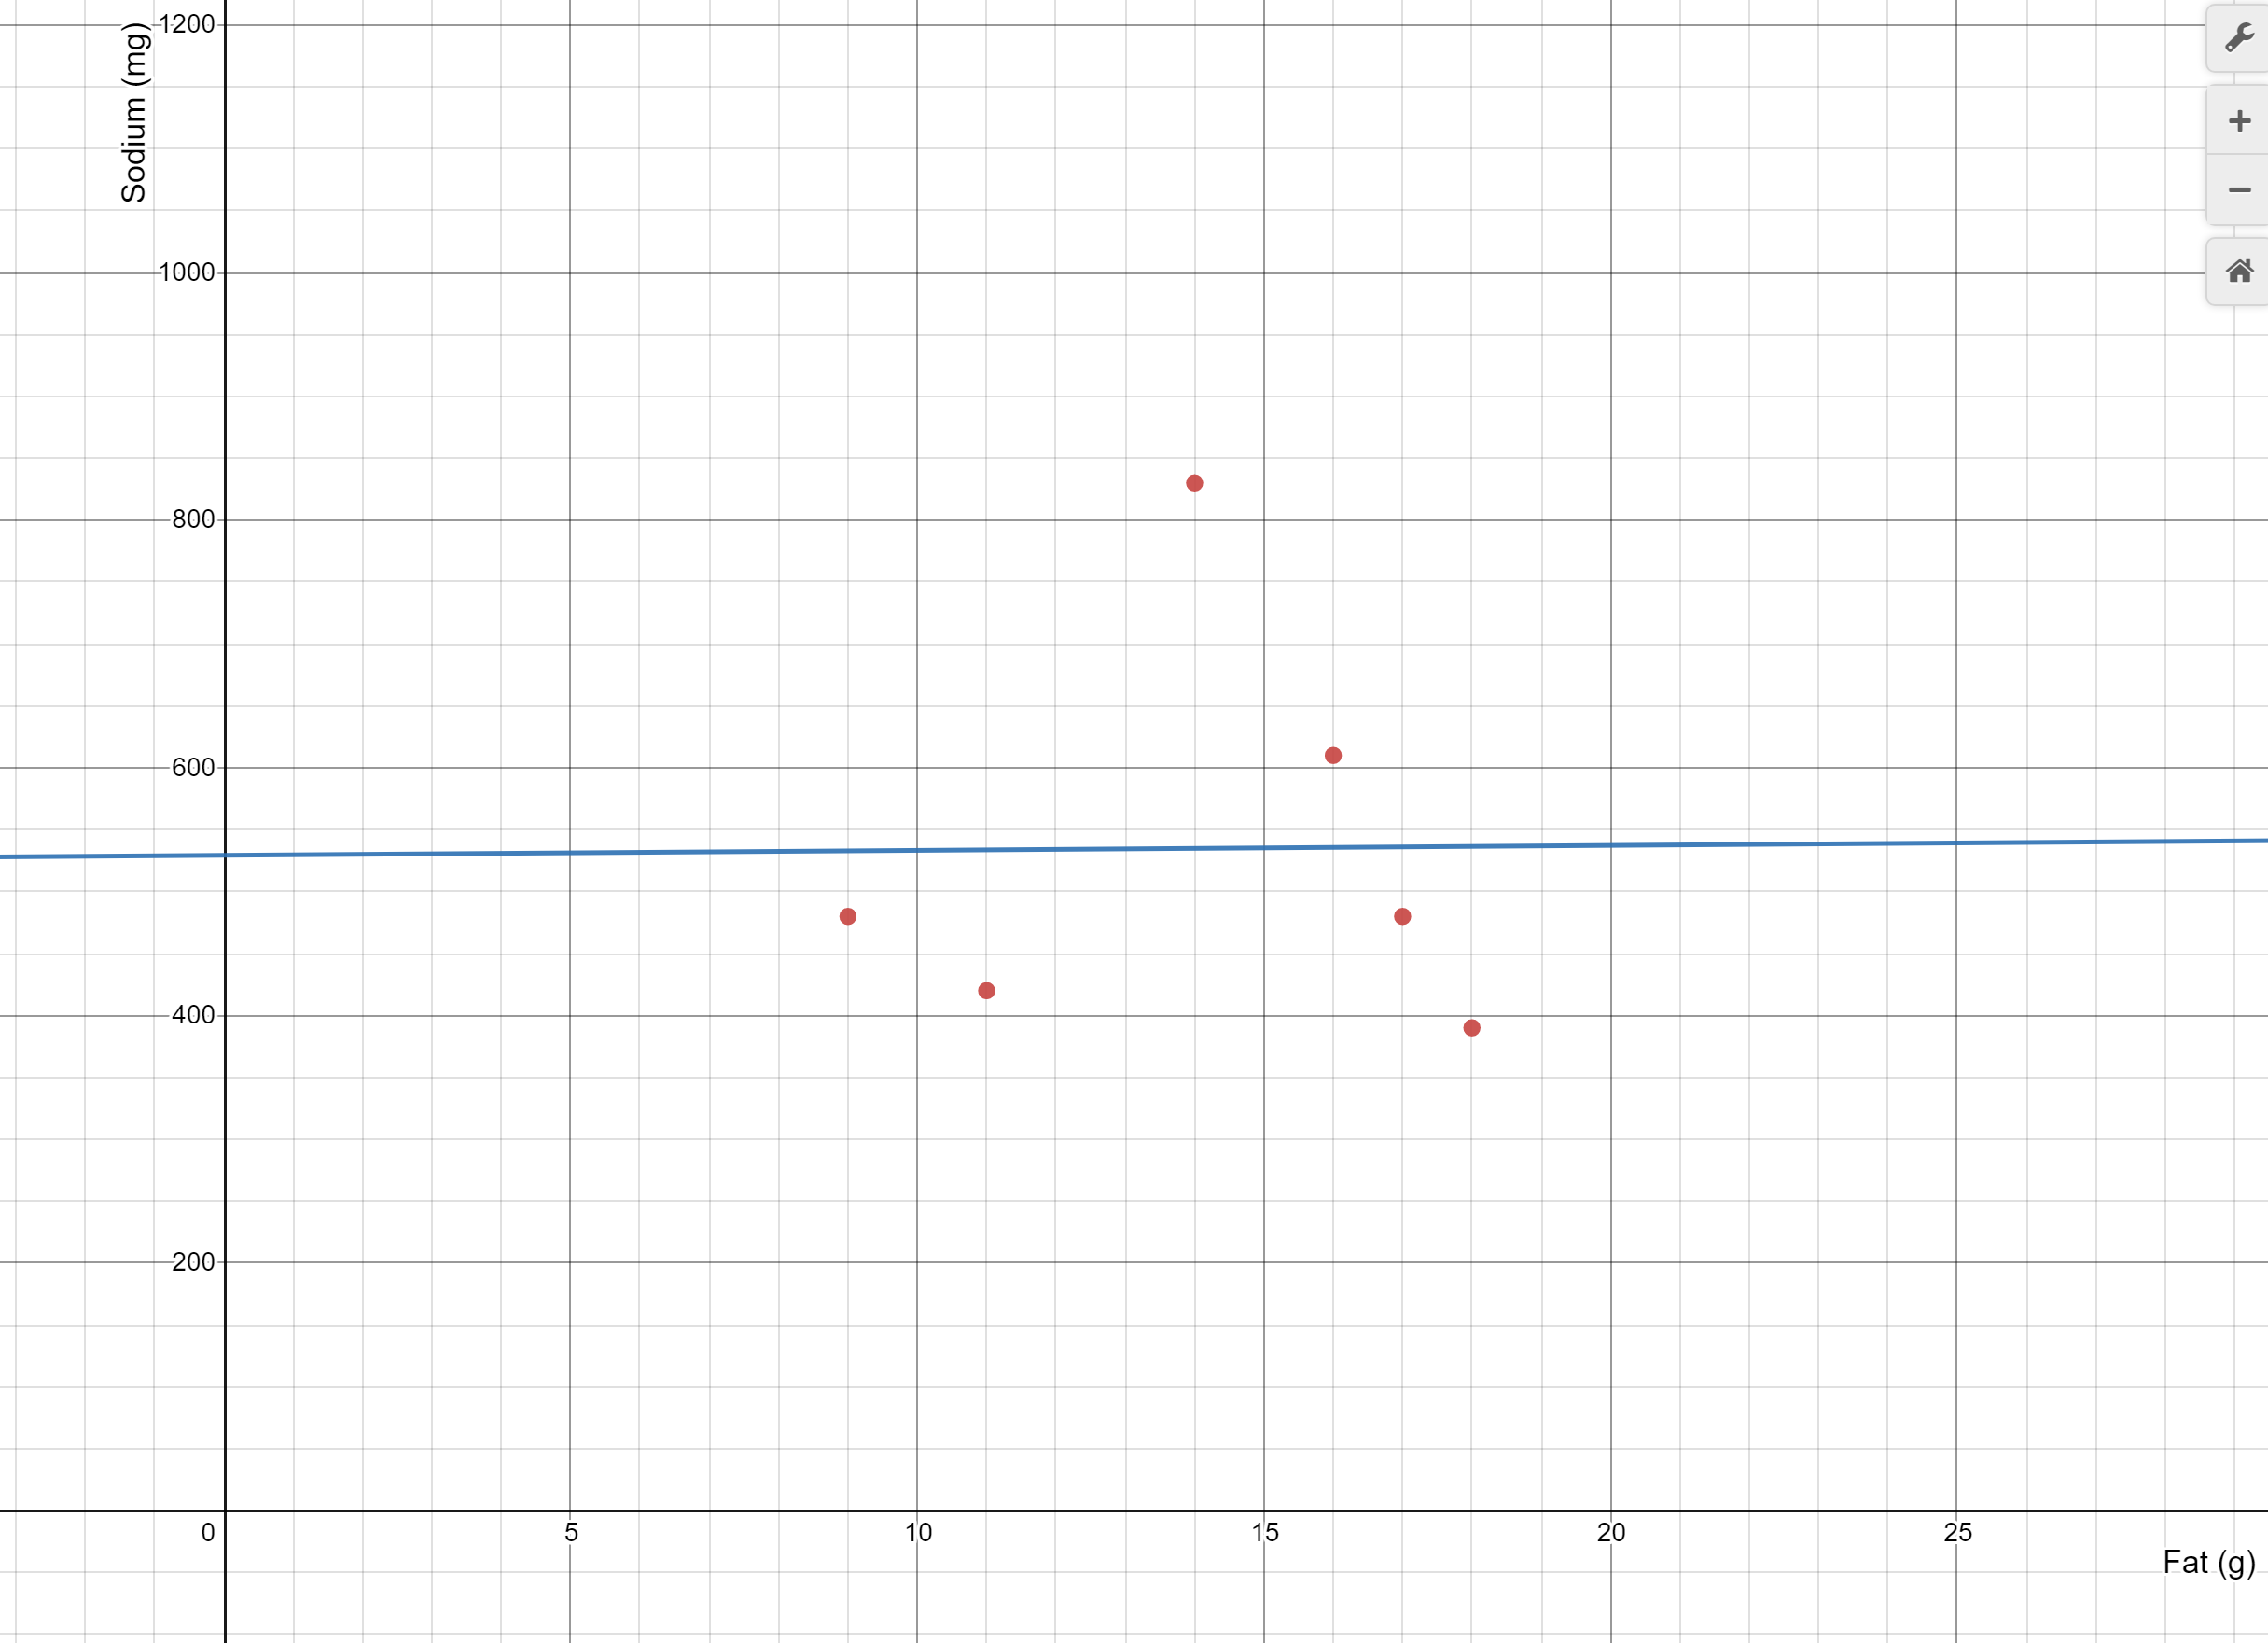
\includegraphics[width=6.75in]{graph.png}
    \end{center}
}
Now, the line does not look as terrible. It could be around 1200 on the y-intercept and about 20 on the x-intercept and go between the set of points to be a bit more accurate. If $(11, 420)$ is an outlier, then a quadratic regression could be useful with a maximum around $(14,800)$. The right cluster looks very linear, but there is some weird shear between the 2nd and 3rd points (from left to right). That, or there is just no correlation between these with any regression curve and it is just a coincidence that the right cluster is linear.
\end{enumerate}
    \newpage
    \item American culture is focused on fat intake as corresponding to a high-calorie diet.
\begin{enumerate}[label=(\alph*)]
    \item Compute the least squares regression line with response variable calorie count
    and input variable fat content. Clearly state sums of the intermediate calculations: $\bar{x},\bar{y},S_{xy},S_{xx}$.

    \nl \textbf{Solution: } Our $x$ represents the fat content, and $y$ is the calorie count. Hence,
    \notab{\begin{align*}
        \bar x &= \over{n} \sum_{i=1}^n x_i = \frac{18 + 11 + 9 + 17 + 14 + 16}{6}
        = 14.1\overline6\\
        %
        \bar y &= \over{n} \sum_{i=1}^n y_i = \frac{310 + 250 + 250 + 390 + 320 + 330}{6}
        = 308.\overline3\\
        %
        S_{xy} &= (18 - 14.1\overline6)(310 - 308.\overline3) + (11 - 14.1\overline6)(250 - 308.\overline3) + (9 - 14.1\overline6)(250 - 308.\overline3)\\ &\quad + (17 - 14.1\overline6)(390 - 308.\overline3) + (14 - 14.1\overline6)(320 - 308.\overline3) + (16 - 14.1\overline6)(330 - 308.\overline3) \\ &= 761.\overline6\\
        %
        S_{yy} &= (310 - 308.\overline3)(310 - 308.\overline3) + (250 - 308.\overline3)(250 - 308.\overline3) + (250 - 308.\overline3)(250 - 308.\overline3) \\ &\quad+ (390 - 308.\overline3)(390 - 308.\overline3) + (320 - 308.\overline3)(320 - 308.\overline3) + (330 - 308.\overline3)(330 - 308.\overline3) \\ &= 14083.\overline3
        %
        \\ S_{xx} &= (18 - 14.1\overline6)^2 + (11 - 14.1\overline6)^2 + (9 - 14.1\overline6)^2  + (17 - 14.1\overline6)^2 + (14 - 14.1\overline6)^2 + (16 - 14.1\overline6)^2 \\ &= 62.8\overline3
        \\ \text{Then} \\
        %
        \widehat{\beta}_1
        &= \frac{S_{xy}}{S_{xx}}
        = \frac{761.\overline6}{62.8\overline3}
        = \frac{4570}{377}
        \approx 12.122015915119363395225464190981432360742705570291777188328912466
        \\ \text{and} \\
        %
        \widehat{\beta}_0
        &= \bar{y} - \widehat{\beta}_1 \bar{x}
        = 308.\overline3 - \frac{4570}{377} \cdot 14.1\overline6
        = \frac{\num{51500}}{377}
        \approx 136.60477453580901856763925729442970822281167108753315649867374005
       \end{align*}}
       Hence $\widehat{y} = \widehat{\beta_0} + \widehat{\beta_1} x = \dfrac{51500 + 4570x}{377}  \approx 136.60477 + 12.12202x$.

       \notab{
    \begin{center}
        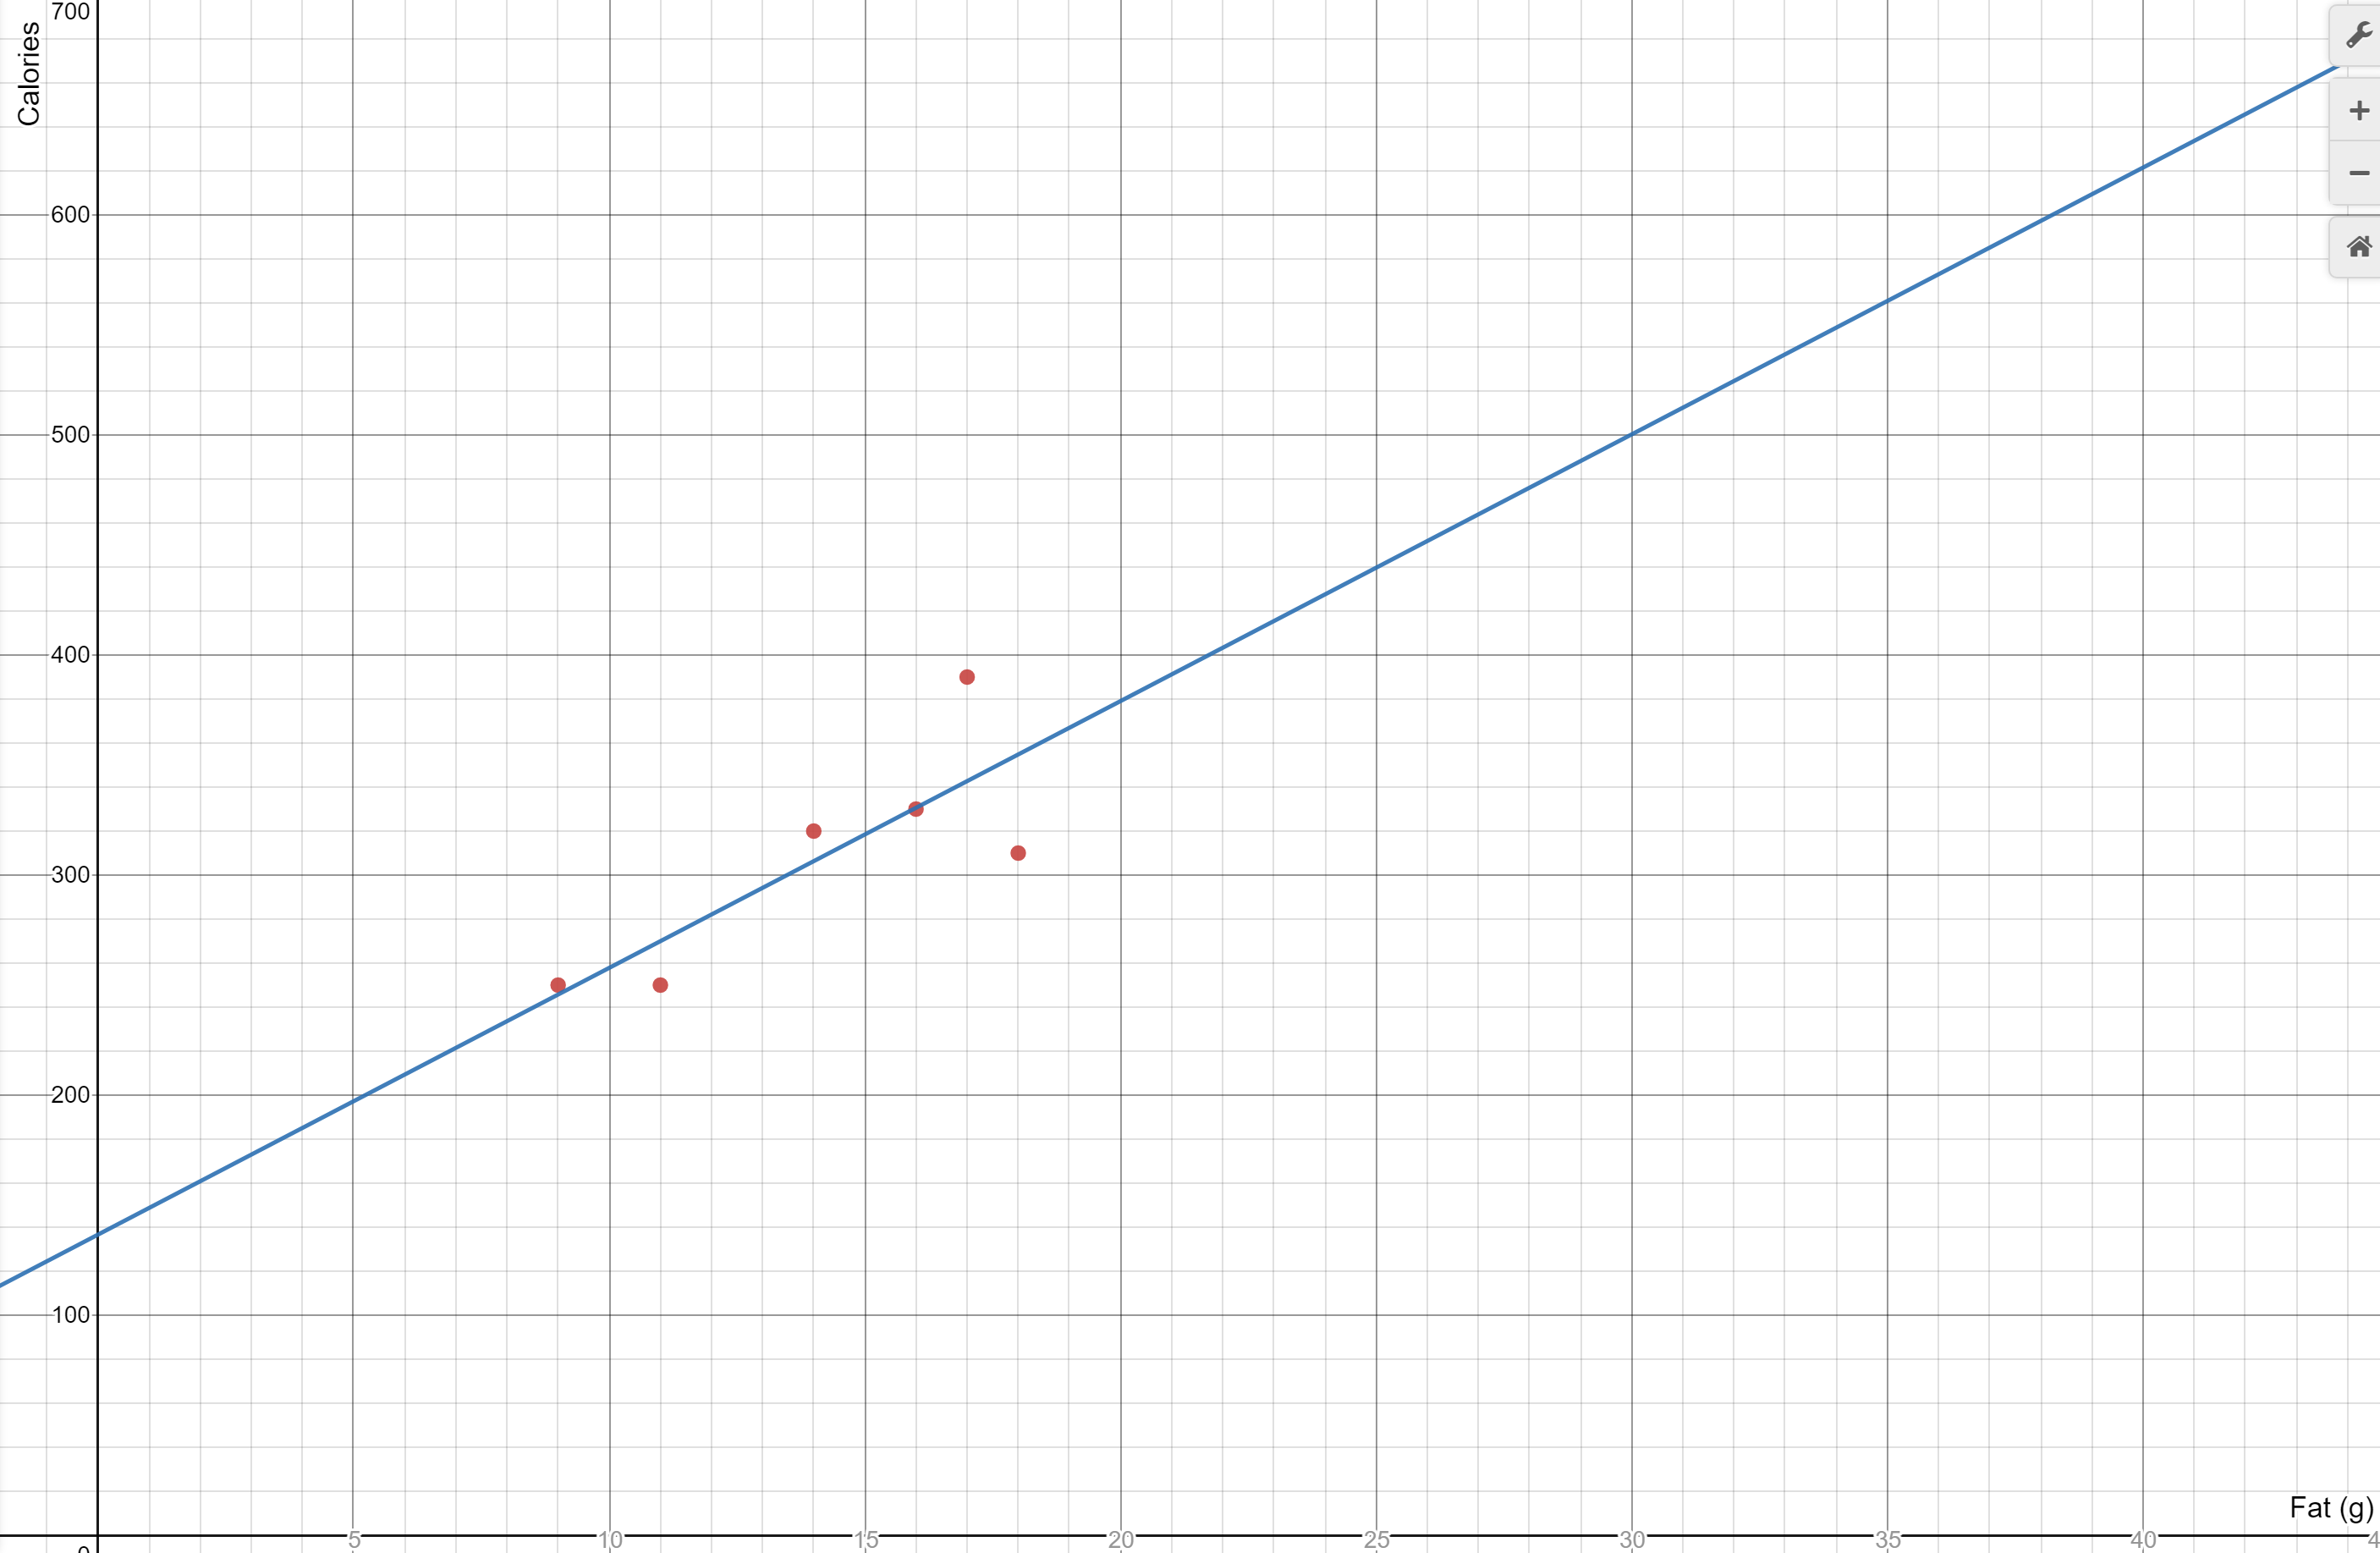
\includegraphics[width=4in]{graph2.png}
    \end{center}
}
    \item Suppose a new burger on the market is known to have 650 calories. What is a good
    estimate for how much fat is in the burger?

    \nl \textbf{Solution: } Since the calorie count is the $y$ value of our regression line, we substitute it in for $y$. Thus,
    \begin{align*}
        & y = 650 = \dfrac{51500 + 4570x}{377} \\
        \iff & 245050 = 51500 + 4570x\\
        \iff & 193550 = 4570x\\
        \iff & x = \frac{19355}{457} \approx 42.352\\
    \end{align*}
    Hence the expected value for the grams of fat in a burger with 650 calories is approximately 42.352 grams. 

 \vspace{1in}
    \item Find an 80\% confidence interval for the slope of the regression line.

\nl \textbf{Solution: } For an 80\% C.I., then $\alpha = 0.2$ and $t_{\alpha/2} = t_{0.1}$. We want to use the formula $I \equiv \widehat{\beta}_i \,\pm\, t_{\alpha/2}(\text{df})\cdot S \sqrt{c_{i\,i}}$. Since the slope coefficient is $\beta_1$ then $i = 1$. 

\nl $t_{0.1}(4) = 1.533$ by Table 5.

\nl $\sqrt{c_{i\,i}} = \sqrt{\dfrac{1}{S_{xx}}} = \sqrt{\dfrac{6}{377}}$ by part (3a).

\nl $\operatorname{SSE} = S_{yy} - \widehat{\beta}_1 \cdot S_{xy} = \dfrac{42250}{3} - \dfrac{4570}{377}  \cdot \dfrac{2285}{3} = \dfrac{\num{1828600}}{377} \approx 4850.39788$ from (3a).

\nl $S = \sqrt{\dfrac{1}{n-2} \operatorname{SSE}} = \sqrt{\dfrac{1}{6-2} \dfrac{\num{1828600}}{377}} =  \dfrac{5\sqrt{\num{6893822}}}{377} \approx 34.822399$ by above.

\nnl Substituting in the respective values, then
\begin{align*}
    \widehat{\beta}_1 \,\pm\, t_{\alpha/2}(\text{df})\cdot S \sqrt{c_{1\,1}} &= \frac{4570}{377} \,\pm\, 1.533 \cdot \dfrac{5\sqrt{\num{6893822}}}{377} \cdot \sqrt{\dfrac{6}{377}}  \\
    &= \frac{4570}{377} \,\pm\, \dfrac{15.33\sqrt{27429}}{377}\\
    &= \dfrac{4570 \pm 15.33\sqrt{27429}}{377}
\end{align*}
$$\text{C.I.} = \pars{\dfrac{4570 - 15.33\sqrt{27429}}{377}, \quad \dfrac{4570 + 15.33\sqrt{27429}}{377}}$$
$$\text{C.I.} \approx \pars{5.387509175, \, 18.85652265}$$
    \item Is there statistical evidence that the slope of the regression line is greater than 10?
    Run a hypotheses test at $\alpha = 0.05$.


    \nl \textbf{Solution: } Let $H_0 : \beta_1 = 10$ and $H_a : \beta_1 > 10$. Then our one-sided $t$-value is $t_{\alpha}(\text{df}) = t_{0.05}(4) = 2.132$.

    \nl Then the $\mathcal T$ statistic is defined as
    \begin{align*}
        \mathcal T &= \frac{\widehat{\beta}_1 - \beta_1}{S\sqrt{c_{1\,1}}} \\
        &= \frac{ \dfrac{4570}{377} - 10}{\dfrac{5\sqrt{6893822}}{377} \sqrt{\dfrac{6}{377}}}\\
        &= \frac{377 \pars{ \dfrac{4570}{377} - 10}}{10\sqrt{27429}}\\
        &= \frac{80\sqrt{27429}}{27429}\\
        &\approx 0.483042.
    \end{align*}
    Then $\Pr \pars{\mathcal T < t} \approx 0.327157$ by webassign technology ($t$-distribution, right tail, \\$\mathcal T = 0.4830$, $\text{df} = 4$). Since $p > \alpha$ then we accept the null hypothesis. Hence, there is \textbf{not} enough statistical evidence that the slope is greater than 10.
\end{enumerate}
    \end{enumerate}
\end{document} 